\subsection{Loewner Framework ROM}

\begin{frame}{Loewner Method Motivation}
The projection based ROM works very well, as proven by the error plot. What do we need the Loewner Method for?\\
\bigskip
Reasons:
\begin{itemize}
    \item To use the projection method, need {\bf A},{\bf b},{\bf c},{\bf d}, and {\bf E}
    \item In some applications, matrices not given
    \item Can be used with only transfer function data
    \item Retains interpolation property, mimics projection method
\end{itemize}
\bigskip
Downsides:
\begin{itemize}
    \item Loewner matrices might become singular if too many sample frequencies are used
    \item Which frequencies to sample data from?
    \item Needs {\bf d} in FOM
\end{itemize}
    
\end{frame}

%%%%%%%%%%%%%%%%%%%%%%%%%%%%%
\begin{frame}{Loewner Data Setup}
First, lets assume that in the FOM ${\bf d} =0$\\
\bigskip
Left frequencies:
\begin{align*}
    {\bf \Sigma} &= \{\sigma_1, \dots, \sigma_r\} \subset \mathbb{I}
\end{align*}
\\
Right frequencies:
\begin{align*}
    {\bf \Theta} &= \{\theta_1, \dots, \theta_r\} \subset \mathbb{I}
\end{align*}

with

$${\bf \Sigma} \cap {\bf \Theta} = \emptyset$$

\end{frame}
%%%%%%%%%%%%%%%%%%%%%%%%%%%%%%%%%%%%%%%%%%%%%%%%%%%%%%%%%%%%%%%%%%%%%%%%%%%%%%%%%%%%%%
\begin{frame}{Loewner Matrices and ROM}

Construct the Loewner Matrix:
\begin{align*}
    \mathbb{L}_{ij} &=  \frac{{\bf H}(\sigma_i)-{\bf H}(\theta_j)}{\sigma_i - \theta_j}\\
\end{align*}
Construct the Shifted Loewner Matrix:
\begin{align*}
    \mathbb{M}_{ij} &= \frac{\sigma_i{\bf H}(\sigma_i)-\theta_j{\bf H}(\theta_j)}{\sigma_i - \theta_j}\\
\end{align*}

\end{frame}
%%%%%%%%%%%%%%%%%%%%%%%%%%%%%%%%%%%%%%%%%%%%%%%%%%%%%%%%%%%%%%%%%%%%%%%%%%%%%%%%%%%%%%
\begin{frame}{Loewner Matrices and ROM}
Construct the Loewner ROM:

\begin{align*}
    {\bf \widehat{A} } & = -\mathbb{M} \\
    {\bf \widehat{b} } & = \left[{\bf H}(\sigma_1), \dots, {\bf H}(\sigma_r) \right]^T\\
    {\bf \widehat{c}}^T & = \left[{\bf H}(\theta_1), \dots, {\bf H}(\theta_r) \right]\\
    {\bf \widehat{E} } & = -\mathbb{L}\\
    {\bf \widehat{d} } & = 0 \\ \\
    {\bf \widehat{H}}(s) & = {\bf \widehat{c}}^T \big( s{\bf \widehat{E}}-{\bf \widehat{A}} \big)^{-1} {\bf \widehat{b}} + {\bf \widehat{d}}
\end{align*}


\end{frame}

%%%%%%%%%%%%%%%%%%%%%%%%%%%%%%%%%%%%%%%%%%%%%%%%%%%%%

\begin{frame}{Loewner Interpolation Theorem}

\begin{theorem}
Assume $\mathbb{M}-s\mathbb{L}$ is invertible for all $s \in \Sigma \cup \Theta$.\\
\bigskip
Then, the previously described ROM transfer function interpolates at the left and right training frequencies:\\
\bigskip
${\bf H}(s) = {\bf \widehat H}(s)$ for all $s \in \Sigma \cup \Theta$
\end{theorem}

\end{frame}
%%%%%%%%%%%%%%%%%%%%%%%%%%%%%%%%%%%%%%%%%%%%%%%%%%%%%%%%%%
\begin{frame}{Loewner Interpolation Property Proof}

Simplify the constructed Loewner ROM 
\begin{align*}
{\bf \widehat{H}}(s) & = {\bf \widehat{c}}^T \big( s{\bf \widehat{E}}-{\bf \widehat{A}} \big)^{-1} {\bf \widehat{b}} \\
{\bf \widehat{H}}(s) &= \left[{\bf H}(\theta_1), \dots, {\bf H}(\theta_r) \right](\mathbb{M} - s \mathbb{L})^{-1} \left[{\bf H}(\sigma_1), \dots, {\bf H}(\sigma_r) \right]^T
\end{align*}

Consider the matrix $\mathbb{M} - s \mathbb{L}$ where $s \in \mathbb{C}$.\\
\bigskip
$$(\mathbb{M} - s \mathbb{L})_{i,j} = \frac{s - \theta_j}{\sigma_i - \theta_j}{\bf H}(\theta_j) + \frac{\sigma_i - s}{\sigma_i - \theta_j}{\bf H}(\sigma_i)$$\\

\bigskip

Two interpolatory cases for s:

\begin{enumerate}
    \item $s = \theta_k$ for some k
    \item $s = \sigma_k$ for some k
\end{enumerate}

\end{frame}

%%%%%%%%%%%%%%%%%%%%%%%%%%%%%%%%%%%%%%%%%%%%%%
\begin{frame}{Loewner Interpolation Property Proof}

Consider case where $s = \theta_k$.\\
\bigskip
Recall:
$$(\mathbb{M} - s \mathbb{L})_{i,j} = \frac{s - \theta_j}{\sigma_i - \theta_j}{\bf H}(\theta_j) + \frac{\sigma_i - s}{\sigma_i - \theta_j}{\bf H}(\sigma_i)$$

\begin{center}
$(\mathbb{M} - \theta_k \mathbb{L})e_k = \left[{\bf H}(\sigma_1), \dots, {\bf H}(\sigma_r) \right]^T \implies$ \\
$e_k = (\mathbb{M} - \theta_k \mathbb{L})^{-1}\left[{\bf H}(\sigma_1), \dots, {\bf H}(\sigma_r) \right]^T$
\end{center}

\begin{center}
$\left[{\bf H}(\theta_1), \dots, {\bf H}(\theta_r) \right] e_k = {\bf H}(\theta_k)$\\

$\left[{\bf H}(\theta_1), \dots, {\bf H}(\theta_r) \right] (\mathbb{M} - \theta_k \mathbb{L})^{-1}\left[{\bf H}(\sigma_1), \dots, {\bf H}(\sigma_r) \right]^T = {\bf \widehat H}(\theta_k)$
\end{center}

Therefore, ${\bf H}(\theta_k) = {\bf \widehat H}(\theta_k)$

\end{frame}
%%%%%%%%%%%%%%%%%%%%%%%%%%%%%%%%%%%%%%%%%%%%%%%%%%%%%%%%%%%
\begin{frame}{Loewner Interpolation Property Proof}

Consider case where $s = \sigma_k$.\\
\bigskip
Recall:
$$(\mathbb{M} - s \mathbb{L})_{i,j} = \frac{s - \theta_j}{\sigma_i - \theta_j}{\bf H}(\theta_j) + \frac{\sigma_i - s}{\sigma_i - \theta_j}{\bf H}(\sigma_i)$$


\begin{center}
$e_k^T(\mathbb{M} - \sigma_k \mathbb{L}) = \left[{\bf H}(\theta_1), \dots, {\bf H}(\theta_r) \right] \implies$ \\
$e_k^T = \left[{\bf H}(\theta_1), \dots, {\bf H}(\theta_r) \right] (\mathbb{M} - \sigma_k \mathbb{L})^{-1}$
\end{center}

\begin{center}
$e_k^T \left[{\bf H}(\sigma_1), \dots, {\bf H}(\sigma_r) \right]^T = {\bf H}(\sigma_k)$\\

$\left[{\bf H}(\theta_1), \dots, {\bf H}(\theta_r) \right] (\mathbb{M} - \sigma_k \mathbb{L})^{-1}\left[{\bf H}(\sigma_1), \dots, {\bf H}(\sigma_r) \right]^T = {\bf \widehat H}(\sigma_k)$
\end{center}

Therefore, ${\bf H}(\sigma_k) = {\bf \widehat H}(\sigma_k)$

\end{frame}

%%%%%%%%%%%%%%%%%%%%%%%%%%%%%%%%%%%%%%%%%%%%%%%%%%%%%%%%%%%%%%%%
\begin{frame}{Dealing with Singular Loewner Matrices}

Necessary that Loewner matrices are nonsingular\\

\bigskip

\begin{itemize}
    \item More frequencies leads to singular Loewner matrices
    \item ROM transfer function will be undefined 
\end{itemize}

\bigskip
Use SVD to extract independent columns of matrices:
\\
\begin{align*}
\bf U_1 \Sigma_1 V_1^* &= \left[ \mathbb{L} \; \mathbb{M} \right] \\
\bf U_2 \Sigma_2 V_2^* &= \left[ \mathbb{L} \; \mathbb{M} \right]^T 
\end{align*}

Given a tolerance for the normalized singular values, let \(k_1, k_2 =\) number of normalized singular values \(>\) the tolerance. Set k = max(\(k_v, k_w\)).\\
\bigskip
Let $\bf U = U_{1k}$ and $\bf V = V_{2k}$.
\end{frame}

%%%%%%%%%%%%%%%%%%%%%%%%%%%%%%%%%%%%%%%%%%%%%%%%%%%%%%%%%%%%%%%%

\begin{frame}{Dealing with Singular Loewner Matrices}

Construct the new Loewner ROM as:

\begin{align*}
    {\bf \widehat{A} } & = {\bf-U^*\mathbb{M}V}\\
    {\bf \widehat{b} } & = {\bf U^*} \left[{\bf H}(\sigma_1), \dots, {\bf H}(\sigma_r) \right]^T\\
    {\bf \widehat{c}}^T & = \left[{\bf H}(\theta_1), \dots, {\bf H}(\theta_r) \right]{\bf V} \\
    {\bf \widehat{E} } & = {\bf -U^*\mathbb{L} V}\\
    {\bf \widehat{d} } & = 0 \\ \\
    {\bf \widehat{H}}(s) & = {\bf \widehat{c}}^T \big( s{\bf \widehat{E}}-{\bf \widehat{A}} \big)^{-1} {\bf \widehat{b}} + {\bf \widehat{d}}
\end{align*}
    
Interpolatory properties of the new Loewner ROM are beyond the scope of this presentation    
\end{frame}
%%%%%%%%%%%%%%%%%%%%%%%%%%%%%%%%%%%%%%%%%%%%%%%%%%
\begin{frame}{Lowner Framework Implementation}

\begin{enumerate}
    \item Choose disjoint imaginary left and right frequencies $\{\sigma_1, \dots, \sigma_r\}$ and $\{\theta_1, \dots, \theta_r\}$, respectively
    \item Compute $\mathbb{L}$ and $\mathbb{M}$
    \begin{itemize}
        \item $\mathbb{L}_{ij} =  \frac{{\bf H}(\sigma_i)-{\bf H}(\theta_j)}{\sigma_i - \theta_j}$
        \item $\mathbb{M}_{ij} = \frac{\sigma_i{\bf H}(\sigma_i)-\theta_j{\bf H}(\theta_j)}{\sigma_i - \theta_j}$
    \end{itemize}
    \item Compute $\bf U$ and $\bf V$ from the SVD of the Loewner pencils
    \item Use the Loewner matrices, $\bf U$, $\bf V$, and the left and right transfer function data to compute the ROM  
\end{enumerate}


\end{frame}
%%%%%%%%%%%%%%%%%%%%%%%%%%%%%%%%%%%%%%%%%%%%%%%%%%%%%%%%%%%%%%%%
\begin{frame}{Actual H(s) vs Loewner H(s)}

Using 5 left and 5 right frequencies:

\centering
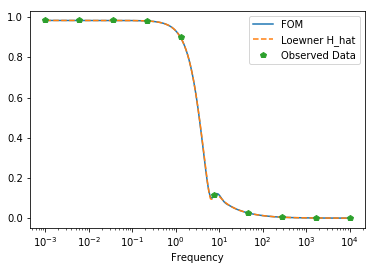
\includegraphics[width=5cm, height= 4cm]{figures/loewner2.png}
\bigskip
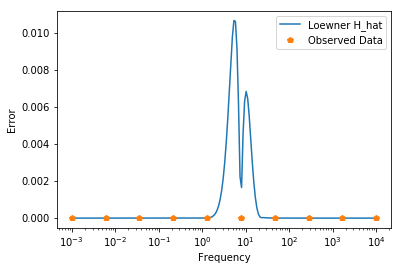
\includegraphics[width=5cm, height=4cm]{figures/loewner1.png}

\end{frame}
%%%%%%%%%%%%%%%%%%%%%%%%%%%%%%%%%%%%%%%%%%
\begin{frame}{Converting Loewner to Real}

Since the right and left frequencies are complex, the ouput of the transfer function at these frequencies will be complex as well. This leads to complex Loewner matrices.\\
\bigskip
The original problem is in the time domain.\\
\bigskip
\begin{itemize}
    \item <1-> Need real matrices $\bf \widehat A$, $\bf \widehat b$, $\bf \widehat c$, $\bf \widehat d$, and $\bf \widehat E$\\
\end{itemize}
\bigskip
Compute real $\mathbb{L}$ and $\mathbb{M}$
\bigskip
\begin{itemize}
    \item <1-> Problem:
    \begin{itemize}
        \item How do we retain the info in $\mathbb{L}$, $\mathbb{M}$?
    \end{itemize}
\end{itemize}
\bigskip
Utilize the fact that $\overline{\bf{H}(s)} = \bf{H}(\overline{s})$.

\end{frame}

%%%%%%%%%%%%%%%%%%%%%%%%%%%%%%%%%%%%%%%%%%%%%%%%%%
\begin{frame}{Converting Loewner to Real}

First include the complex conjugate data in the setup.\\
\bigskip
Left frequencies:
\begin{align*}
    {\bf \Sigma} &= \{\sigma_1, \dots, \sigma_{2r}\} \subset \mathbb{I}
\end{align*}
where $\sigma_{2i} = \overline \sigma_{2i-1}$\\
\bigskip
Right frequencies:
\begin{align*}
    {\bf \Theta} &= \{\theta_1, \dots, \theta_{2r}\} \subset \mathbb{I}
\end{align*}
where $\theta_{2i} = \overline \theta_{2i-1}$\\

\end{frame}
%%%%%%%%%%%%%%%%%%%%%%%%%%%%%%%%%%%%%%%%%%%%%%%%%%
\begin{frame}{Converting Loewner to Real}

Let ${\bf J} \in \mathbb{C}^{n \times n}$ be a block diagonal matrix with $\frac{1}{\sqrt 2}\begin{bmatrix} 1 & -i\\ 1 & i\end{bmatrix}$ repeated on the diagonal.\\
\bigskip
Use the following real Loewner matrices to compute ${\bf U}_R$ and ${\bf V}_R$:
\begin{align*}
    \mathbb{L}_R &= {\bf J}^* \mathbb{L} {\bf J}\\
    \mathbb{M}_R &= {\bf J}^* \mathbb{M} {\bf J}\\
\end{align*}


\end{frame}
%%%%%%%%%%%%%%%%%%%%%%%%%%%%%%%%%%%%%%%%%%%%%
\begin{frame}{Converting Loewner to Real}

Construct the real Loewner ROM as:

\begin{align*}
    {\bf \widehat{A} } & = -{\bf U}_R^T \mathbb{M}_R {\bf V}_R\\
    {\bf \widehat{b} } & = {\bf U}^T {\bf J}^* \left[{\bf H}(\sigma_1), \dots, {\bf H}(\sigma_r) \right]^T\\
    {\bf \widehat{c}}^T & = \left[{\bf H}(\theta_1), \dots, {\bf H}(\theta_r) \right] {\bf J} {\bf V} \\
    {\bf \widehat{E} } & = -{\bf U}_R^T \mathbb{L}_R {\bf V}_R\\
    {\bf \widehat{d} } & = 0 \\ \\
    {\bf \widehat{H}}(s) & = {\bf \widehat{c}}^T \big( s{\bf \widehat{E}}-{\bf \widehat{A}} \big)^{-1} {\bf \widehat{b}} + {\bf \widehat{d}}
\end{align*}

\end{frame}
%%%%%%%%%%%%%%%%%%%%%%%%%%%%%%%%%%%%%%%
\begin{frame}{How does this work?}

Consider computing $\mathbb{L}_R$ in the case where $\Sigma = \{\sigma, \overline \sigma\}$ and $\Theta = \{\theta, \overline \theta\}$:\\
\begin{align*}
\mathbb{L}_R &= \frac{1}{2} \begin{bmatrix} 1 & 1\\ i & -i \end{bmatrix}
\begin{bmatrix} \frac{{\bf H}(\sigma) - {\bf H}(\theta)}{\sigma - \theta} & \frac{\overline{{\bf H}(\sigma)} - {\bf H}(\theta)}{\overline \sigma - \theta}\\[1em] \frac{{\bf H}(\sigma) - \overline{{\bf H}(\theta)}}{\sigma - \overline \theta} & \frac{\overline{{\bf H}(\sigma)} - \overline{{\bf H}(\theta)}}{\overline \sigma - \overline \theta} \end{bmatrix}
\begin{bmatrix} 1 & -i\\ 1 & i\end{bmatrix}\\[1em]
\mathbb{L}_R &= \begin{bmatrix} re(\frac{{\bf H}(\sigma) - {\bf H}(\theta)}{\sigma - \theta}) & im(\frac{{\bf H}(\sigma) - {\bf H}(\theta)}{\sigma - \theta}) \\[1em] -im(\frac{{\bf H}(\sigma) - {\bf H}(\theta)}{\sigma - \theta}) & re(\frac{{\bf H}(\sigma) - {\bf H}(\theta)}{\sigma - \theta})\end{bmatrix}
\end{align*}

The matrix $\mathbb{L}_R$ is real but encapsulates the same information as the complex number $\frac{{\bf H}(\sigma) - {\bf H}(\theta)}{\sigma - \theta}$.\\
\bigskip
Same holds for $\mathbb{M}_R$.
\end{frame}